% This is "sig-alternate.tex" V2.1 April 2013
% This file should be compiled with V2.5 of "sig-alternate.cls" May 2012
%
% ----------------------------------------------------------------------------------------------------------------
% This .tex file (and associated .cls V2.5) produces:
%       1) The Permission Statement
%       2) The Conference (location) Info information
%       3) The Copyright Line with ACM data
%       4) NO page numbers
%
% as against the acm_proc_article-sp.cls file which
% DOES NOT produce 1) thru' 3) above.
%
% Using 'sig-alternate.cls' you have control, however, from within
% the source .tex file, over both the CopyrightYear
% (defaulted to 200X) and the ACM Copyright Data
% (defaulted to X-XXXXX-XX-X/XX/XX).
% e.g.
% \CopyrightYear{2007} will cause 2007 to appear in the copyright line.
% \crdata{0-12345-67-8/90/12} will cause 0-12345-67-8/90/12 to appear in the copyright line.
%
% ---------------------------------------------------------------------------------------------------------------
% This .tex source is an example which *does* use
% the .bib file (from which the .bbl file % is produced).
% REMEMBER HOWEVER: After having produced the .bbl file,
% and prior to final submission, you *NEED* to 'insert'
% your .bbl file into your source .tex file so as to provide
% ONE 'self-contained' source file.
%
% For tracking purposes - this is V2.0 - May 2012

\documentclass[sigconf]{acmart}

\usepackage{multirow}
\usepackage{graphicx}
\DeclareGraphicsExtensions{.pdf,.png}
\graphicspath{{./figures/}}

\usepackage{amssymb}
\usepackage{amsmath}
\usepackage{color}

% Copyright
\setcopyright{acmcopyright}
%\setcopyright{acmlicensed}
%\setcopyright{rightsretained}
%\setcopyright{usgov}
%\setcopyright{usgovmixed}
%\setcopyright{cagov}
%\setcopyright{cagovmixed}

% DOI
\acmDOI{10.475/123_4}

% ISBN
\acmISBN{123-4567-24-567/08/06}

%Conference
\acmConference[WWW'17]{WWW conference}{April 2017}{Perth, Australia} 
\acmYear{2017}
\copyrightyear{2016}

\acmPrice{15.00}

\begin{document}

%
% --- Author Metadata here ---
%\conferenceinfo{WOODSTOCK}{'97 El Paso, Texas USA}
%\CopyrightYear{2007} % Allows default copyright year (20XX) to be over-ridden - IF NEED BE.
%\crdata{0-12345-67-8/90/01}  % Allows default copyright data (0-89791-88-6/97/05) to be over-ridden - IF NEED BE.
% --- End of Author Metadata ---

\title{Performance Monitoring and Root Cause Analysis for Cloud-hosted Web Applications}

\author{Hiranya Jayathilaka, Chandra Krintz, Rich Wolski}
\affiliation{%
  \institution{Computer Science Department}
  \streetaddress{University of California, Santa Barbara}
}
\email{[hiranya,ckrintz,rich]@cs.ucsb.edu}

\begin{abstract}
In this paper, we describe Roots -- a system for automatically identifying the
``root cause'' of performance anomalies in web applications deployed
in Platform-as-a-Service (PaaS) clouds.
Roots does not require
application-level instrumentation.  Instead, it tracks events within the PaaS
cloud that are triggered by application requests using a
combination of metadata injection and platform-level instrumentation.

We describe the extensible Roots architecture, a prototype implementation 
of the system, and a statistical methodology for performance anomaly
detection and diagnosis.  We evaluate the efficacy of Roots
using a set of PaaS-hosted web services, and detail the performance
overhead and scalability of the implementation.


\end{abstract}

\keywords{ACM proceedings, \LaTeX, text tagging}

\maketitle

%
%  Use this command to print the description
%
%\printccsdesc

% We no longer use \terms command
%\terms{Theory}

%\keywords{ACM proceedings; \LaTeX; text tagging}

\section{Introduction}
Over the last decade cloud computing has become a popular approach for
deploying applications at
scale~\cite{Antonopoulos:2010:CCP:1855007,Pinheiro:2014:ACC:2618168.2618188}.
This widespread adoption of cloud computing, particularly for deploying web
applications, is facilitated by ever-deepening software abstractions.  While
abstractions elide much of 
the complexity necessary to enable scale, they also obscure
the runtime details, making the diagnosis of performance
problems challenging.  Therefore, the rapid expansion of cloud technologies
combined with their increasing opacity has intensified the need for new
techniques to monitor applications deployed in cloud
platforms~\cite{DaCunhaRodrigues:2016:MCC:2851613.2851619}. 

Application developers and cloud administrators wish to monitor
application performance, detect anomalies, and identify performance 
bottlenecks. To
obtain this level of operational insight in a cloud,
the cloud platform must support data gathering and analysis capabilities that
span the entire software stack.  However, most cloud technologies
available today do not provide adequate means to monitor applications or the cloud
services they depend on, in a way that facilitates identifying performance bottlenecks
within the cloud platform.

Application-level instrumentation packages are
plentiful~\cite{newrelic,datadog,dynatrace}, but because they perturb the
applications they can significantly increase the
effort and financial cost of application development and maintenance.  Moreover, cloud
administrators must trust the application developers to instrument their
applications correctly (e.g. logging all the relevant 
information to diagnose a rare performance fault).  Even when good application
instrumentation is available, however, because applications depend 
so heavily on extant performance opaque
cloud services (e.g. database services, in-memory caching, etc.),
it is often difficult, if not impossible, to diagnose
the ``root cause'' of a performance problem.

%Cloud
%administrators must therefore trust the application developers to implement
%necessary logging and instrumentation at the application level. This typically
%entails using third party, external monitoring
%software~\cite{newrelic,datadog,dynatrace}, which significantly increases the
%effort and financial cost of maintaining applications.  Developers must also
%ensure that their instrumentation is both correct, and does not degrade
%application performance.  Nevertheless, since the applications depend on
%extant cloud services (e.g. database services, in-memory caching, etc.) that
%are performance-opaque, it is often difficult, if not impossible to diagnose
%the ``root cause'' of a performance problem using extrinsic forms of
%monitoring.

%reporting application performance.
%
%only provide primitive
%monitoring features such as application-level logging. Hence, their support for performance
%anomaly detection and bottleneck identification is severely limited.

Further compounding the performance
diagnosis problem, today's cloud platforms are 
large and complex~\cite{DaCunhaRodrigues:2016:MCC:2851613.2851619,Ibidunmoye:2015:PAD:2808687.2791120}. 
They are
comprised of many layers, where each layer may consist of many interacting components.
Therefore when a performance anomaly manifests in a user application, it is
often challenging
to determine the exact software component that is responsible. 
Facilitating this type root cause analysis requires
both data collection at different layers of the cloud, and mechanisms for correlating 
the events recorded at different layers~\cite{7420511}. 
%
%Today's cloud platforms do not support such fine-grained
%data collection across the board. 
%
%The plethora of existing third party cloud monitoring solutions
%do not have visibility into the low-level activities of the cloud thereby rendering them incapable
%of performing systemwide root cause analysis.

%Moreover, performance monitoring for cloud applications needs to be highly customizable. Different
%applications have different monitoring requirements in terms of data gathering frequency (sampling rate), 
%length of the history to consider when performing statistical analysis (sample size), and the performance 
%SLOs (service level objectives~\cite{XXX}) that govern the application.
%%to maintain over time and check for
%%violations. 
%Cloud monitoring should be able to facilitate these diverse requirements on a
%per-application basis.
%Designing such customizable and extensible performance
%monitoring frameworks that are built into the cloud platforms is a novel and challenging undertaking.

In this paper, we present \textit{Roots} --  
a full-stack application platform 
monitor (APM) that is designed to be integrated
into a variety of cloud Platform-as-a-Service (PaaS) technologies. 
PaaS clouds, in particular, provide abstractions that hide most of the 
details concerning application
runtime~\cite{Soni:2014:CCB:2592737.2592741}. 
They offer a set of scalable, managed cloud services that
provide an assortment of functionality,
which developers invoke from the application implementations.
%to compose 
%into applications.
%The implementation and deployment details of these services are completely opaque to the developers. 
%However, the existing cloud monitoring techniques rely on being able to capture data from all components 
%of an application, all the way down to the virtual machines that host them. Such methods are
%therefore not viable in a PaaS cloud that hides runtime details beneath a layer of managed services.
To be able to correlate application activity with cloud service events,
Roots must be able to introspect the entire platform software stack. Therefore we
have chosen to design it
%we design Roots 
as another managed service built into the PaaS cloud. 
%Therefore
%it operates at the same level as the other services offered by the cloud platform. This way Roots can collect data
%directly from the internal service implementations of the cloud platform, thus gaining full visibility into all the 
%inner workings of an application. 
As an added benefit, by implementing Roots as an intrinsic PaaS service,
%It also enables Roots to 
it can function fully automatically in the background, without
requiring instrumentation of application code. Instead,
Roots intercepts and records events as the
application code invokes various service implementations of the PaaS cloud,
and then correlates them with specific application requests.
Roots also records the latency of each application request, and
of each application call to an
internal cloud service implementation. %It uses batch operations and asynchronous 
%communication to record events with the goal of introducing minimal overhead.

%The proposed
%APM is not an external system that monitors a cloud platform from the outside (as most APM systems today). 
%Rather, it integrates with
%the PaaS cloud from within thereby extending and augmenting the existing components of the PaaS cloud
%to provide comprehensive full stack monitoring. 
%We believe that this design decision is a key differentiator over existing cloud 
%application monitoring systems because (i) it is
%able to take advantage of the scaling, efficiency, deployment, fault tolerance, security, 
%and control features that the underlying cloud offers, 
%(ii) while providing low overhead end-to-end monitoring of cloud applications.
%
%Previous work has outlined several key requirements that need to be taken into consideration when
%designing a cloud monitoring system~\cite{DaCunhaRodrigues:2016:MCC:2851613.2851619,Ibidunmoye:2015:PAD:2808687.2791120}. 
%We incorporate a number of these features into our design:
%\begin{description}
%\item[Scalability] Roots is lightweight, and does not cause any noticeable overhead in 
%application performance. It also puts strict upper bounds on the volume of data kept in memory. 
%The persistent data is accessed on demand, and can be removed after their usefulness has expired.
%\item[Multitenancy] Roots facilitates configuring monitoring policies at the granularity of individual applications.
%Users can employ different statistical analysis methods to process the monitoring data in ways that are 
%most suitable for their applications.
%\item[Complex application architecture] We design Roots to collect data from the entire cloud stack 
%(load balancers, app servers, built-in PaaS services etc.). Roots is able to correlate data gathered
%from different parts of the cloud platform, and perform systemwide bottleneck identification.
%\item[Dynamic resource management] Cloud platforms are dynamic in terms of their magnitude 
%and topology. By augmenting all the key components along the request processing path of the cloud platform,
%we make sure that Roots capture all the critical runtime data. When new processes/components
%spring to life in the cloud platform, they inherit the same augmentations, and start reporting to Roots automatically.
%\item[Autonomy] Roots is designed to detect performance anomalies online, without manual intervention.
%When Roots detects a problem, it attempts to automatically identify the root cause by analyzing
%available workload and service invocation data. Data collection begins automatically for new
%applications as they are deployed.
%\end{description}
%

%Roots collects most of the data it requires by direct integration with various internal components 
%of the cloud platform. In addition to high-level metrics like request throughput
%Roots monitors applications by directly integrating with internal PaaS components.
%In addition to high-level metrics such as request throughput
%and latency, 
 %a manner that does not substantively
%increase request latency.
%\textcolor{blue}{The remainder of this paragraph should
%go in Section~\ref{sec:arch}.
%In addition, Roots employs a collection of lightweight  benchmarking
%processes to collect performance data regarding user applications. Both
%the benchmarking processes, and the data analysis processes are executed 
%out of the request processing flow of the cloud platform. Such processes can be
%grouped together, and managed as a single entity called a
%``Roots Pod''. Pods keep minimum state
%information regarding the applications they monitor and analyze. This enables
%a single pod to monitor a large number of applications. Each pod is self-contained,
%and therefore scalability and high availability can be achieved by running multiple pods (sharding),
%and running multiple replicas of the same pod.}

When Roots detects a performance anomaly in application request latency, 
it attempts to
identify the root cause of the anomaly by analyzing the previous workload 
data of the application,
and the performance of the internal PaaS services on which the application depends.
It determines if the detected anomaly was caused by a change in the
application workload (e.g. a sudden spike in the number of client requests), or an internal
bottleneck in the cloud platform (e.g. a slow database query). To facilitate
this analysis we propose a ``bottleneck identification'' methodology
for PaaS clouds. 
Our approach uses a combination of quantile analysis, change point detection
and linear regression. 

We test the efficacy of our approach with a working prototype of 
Roots using the AppScale~\cite{6488671} open source PaaS. 
%We evaluate the feasibility and the 
%efficacy of Roots by conducting a series of empirical trials using our prototype. 
Our results indicate that using information gathered from the entire cloud
stack to parameterize the bottleneck identification algorithm, Roots
makes remarkably accurate diagnoses.
% nearly 100\% of the time. 
We also demonstrate that Roots does not add a significant performance overhead
to the applications, and that a single Roots pod (our encapsulation abstraction for
data analysis processes) can monitor tens of thousands
of applications simultaneously.

Thus we summarize the contributions made by this paper as follows.
\begin{itemize}
\item We describe the architecture of Roots as an intrinsic PaaS
service, which works automatically without depending upon
application instrumentation.
\item We describe a statistical methodology for determining when an
application is experiencing a performance anomaly, and identifying the 
workload change or the cloud service that is responsible for the anomaly.
\item We demonstrate the effectiveness of the approach using a working PaaS
prototype and real web applications.
\end{itemize}

%Rest of this paper is organized as follows.
%Section~\ref{sec:background} sets the stage for introducing Roots by describing the domain of 
%PaaS clouds and discussing performance monitoring fundamentals. Section~\ref{sec:arch} 
%details the high level architecture of Roots along with the motivation behind our design choices.
%Section~\ref{sec:impl} describes our implementation of Roots, with a strong emphasis on our
%solution to the bottleneck identification problem in PaaS clouds. Section~\ref{sec:results} presents our
%experimental results. Then we discuss some related work and conclude. 


\section{Background}
\label{sec:background}
%\textcolor{blue}{You might want to move some of this discussion into the
%introduction since it allows the reader to understand the focus of the work we
%present.}
%Added more details about PaaS services to the intro

%\subsection{The PaaS Model} 

Our work concentrates on the web
applications deployed in PaaS clouds. An application of this nature exposes
one or more web application programming interfaces (web APIs) through which
clients can interact with it. The web APIs accept HTTP/S requests sent by
remote clients, and respond with machine readable responses (e.g. HTML, JSON,
XML, Protocol Buffers~\cite{protobuff}). This type of applications tend to be highly
interactive, and clients typically have strict expectations on the application
response time~\cite{latency-matters}. 
%Studies have shown that poor application response
%time may even lead to revenue loss~\cite{latency-matters}.
Additionally, the PaaS cloud on
which an application is running may impose additional constraints on the
application response time for scalability
reasons~\cite{azure-limits,gae-limits}.  For example Google App Engine
requires that no application request takes more than 60 seconds to execute.

PaaS-hosted web applications, like those that run on Google App Engine
(GAE)~\cite{gae},  
rely on various PaaS kernel services offered by the underlying
cloud platform. 
By offloading common application functionality such as data storage, caching,
user management, and security to a set of scalable and
managed cloud services, application developers
can greatly reduce the amount of code they have to write. 
%It also eliminates the need to install, run and
%manage many other support software that would otherwise be necessary (e.g. a database server, 
%a message broker etc.). 
In other words, when developing applications for a PaaS environment, the
developer simply focuses on implementing his/her application logic
using the available PaaS services to the greatest extent possible.
All the remaining deployment and utility services are left to be handled 
by the PaaS cloud. 

The downside of this approach is that application developers no longer have full runtime visibility
into the application execution. Since most of the application functionality is provided by a set 
of PaaS kernel services that are in cloud provider's domain, the application
developer does not have total control over application performance. If the application 
response time becomes too slow, the application developer is not in a position to determine
where in the entire cloud platform the performance bottleneck is due to the opacity of the cloud
platform's internal implementation. 

One way to circumvent this 
limitation is to instrument application code, and continuously monitor the time taken by various
parts of the application~\cite{newrelic,datadog,dynatrace}. 
But this activity can be tedious for the application developer, 
may be error prone thereby misleading those attempting to
diagnose a problem, and
the additional code instrumentation may slow down or alter the application's
performance. 
%Also there is no way to enforce correct, and consistent instrumentation of application code.  
%That is, the application developers must be careful in gathering and storing the appropriate
%runtime data. Otherwise their analyses will be inaccurate.
Implementing data collection and analysis as a service built into the PaaS cloud allows 
anomaly detection and bottleneck identification to be a ``curated'' service that is 
reliably managed by the cloud platform. The method of using low-level instrumentation
for root cause analysis has already proven effective in IaaS clouds~\cite{Dean:2014:PTR:2696535.2696551}.

\subsection{PaaS Performance Anomalies}

%In this work we define \textit{anomalies} as application performance change events that cause
%one or more performance SLOs to be violated. 

Our model is
one in which the clients of a web application have engaged in a
``service-level agreement'' (SLA)~\cite{Keller:2003:WFS:635430.635442}
with the ``owner'' or operator of the application that is hosted in a PaaS.  The SLA
stipulates a response-time ``service-level objective'' (SLO) that, if violated, constitutes a breech of the
agreement (similar to \cite{Nguyen:2011:PPR:2038633.2038634} but for PaaS).  A performance anomaly, then, is an event or set of events that
causes an application-level SLO to be violated.
%approach associates each application with
%a set of performance SLOs. We consider SLOs concerning the application response time
%(latency), which get violated when an application becomes too slow.
%If the performance of an application deteriorates to the
%point that at least one of its SLOs is violated, we treat it as an anomaly. 

Further, we refer to the process
of diagnosing whether increased workload or an unusually slow software component is responsible for
an anomaly, and in the latter case, the identification of the slow component
as \textit{root cause analysis}.  When request latency increases violating an SLO,
and the workload has not increased, we assume that there is a ``bottleneck''
component in the application code or PaaS runtime that is responsible.  Roots
performs root cause analysis in near real time so
that it can urgently alert cloud users and administrators of the detected problems.
%For a given anomaly, the root cause could be a change in the application workload or
%a \textit{bottleneck} in the application runtime.  Bottlenecks may occur in the application code, 
%or in the PaaS services that the application rely on.

%In order to maintain a satisfactory level of user experience and adhere to any previously
%agreed upon performance SLOs, application developers and cloud administrators wish
%to detect performance anomalies as soon as they occur. When detected, they
%must perform root cause analysis to identify the cause of the anomaly, and take some
%corrective and/or preventive action. 
%This diagnosis usually occurs as a two step process. First, one must determine
%whether the anomaly was caused by a change in the workload (e.g. a sudden 
%increase in the number of client requests). If that is the case,
%the resolution typically involves allocating more resources to the application or spawning
%more instances of the application for load balancing purposes. If the anomaly cannot be 
%attributed to a workload change, one must go another step to find the bottleneck component
%that has given rise to the issue at hand.

%Detecting performance anomalies
%requires continuous monitoring of application performance which could be tedious with
%cloud platforms in use today. It is even more challenging to perform root cause analysis
%due to the complexity and the blackbox nature of the cloud platforms. 

Note that there are several
third party cloud monitoring solutions available today which provide some performance
anomaly detection support~\cite{newrelic,datadog,dynatrace}. 
However, they require additional configuration, are expensive
and cannot support root cause analysis across the entire cloud stack since they do not
have visibility into all components of the cloud.


\section{Approach}
\label{sec:approach}
Our approach is based on the following observations.
\begin{itemize}
\item In a well-designed web application targeted for PaaS environments, 
most of the ``work'' is done by
curated services intrinsic to the PaaS cloud.  
%Put
%another way, if the application is not leveraging the PaaS services to the
%fullest extent, it is not taking advantage of the PaaS model.
\item An application making maximal use of the PaaS services finds that its
performance is defined by the performance of these services.  Since the 
implementation and deployment details of the PaaS services are hidden
from the applications,
performance diagnostics must also be implemented as an intrinsic PaaS service.
\item The integrity and accuracy of application performance diagnostics
cannot rely on programmer-introduced application instrumentation.
\end{itemize}
Thus, the key intuition behind Roots is that as a curated PaaS service
it has visibility into all the activities that occur in various layers of the cloud,
including all invocations of the PaaS kernel services made by the applications.

%Therefore it can automatically collect
% data regarding events that are related to application request processing. 
%The cloud platform can then analyze the collected data offline (but in near realtime) to detect 
%performance anomalies and identify root causes.
%
%We argue that data collection can be implemented efficiently in the cloud platform so as to not
%introduce a significant overhead to deployed applications.
%Moreover, data collection can be always active in the cloud thus relieving the application developers
%from having to instrument their code, or setting up external monitoring.
%The data analysis can benefit from the vast amount of compute
%resources available in the cloud platform. The offline processing ensures that request
%latency is not impacted by monitoring, and the near realtime analysis ensures that developers
%and other interested parties are notified of performance anomalies urgently. 

\subsubsection{Data Collection and Correlation}

Since Roots does not rely on application instrumentation inserted by the
programmer or a third-party tool, it must be able to collect performance data
for a specific application, and correlate application behavior with performance
events occurring within the PaaS services.
Typically, each individual layer of the cloud platform collects data regarding
its own
state changes. It cannot monitor state changes
in other layers without violating the software isolation properties of
layering in general.   That is, layers typically log their own internal
activities, but do not (or cannot is many cases) correlate these activities
with the internal activities of other layers.
 
%There are two issues that need to be addressed when designing a monitoring framework for
%a system as complex as a PaaS cloud.
%\begin{enumerate}
%\item Collecting data from multiple different layers.
%\item Correlating data collected from different layers.
%\end{enumerate}

%However,
%processing an application request involves cooperation of multiple 
%layers. For example, an application request gets routed through the front-end server before
%it reaches the application server. The application server may then invoke one or more PaaS kernel
%services. Depending on how the kernel services are implemented,
%even more layers may get involved in processing the request. 
%In order to facilitate systemwide monitoring and
%bottleneck identification, we should be able to gather data from all the different layers involved
%in processing a request. Then we should be able to correlate the collected data, and tie the events that
%are related to the same request together.

Roots modifies the front-end request server (typically a software load
balancer) 
%To facilitate these requirements, we start by augmenting the front-end server of the cloud platform. 
%Specifically we get the front-end server 
to tag all incoming application requests with unique identifiers.
This request identifier can be attached to an HTTP request as a header, which is visible to all 
internal components of the PaaS cloud. Then we configure the data collecting
agents associated with each software layer in the PaaS 
platform to record the request identifiers along with any events they capture. 
This way we maintain the relationship between application requests, and the resulting
local state changes in different layers of the cloud, without breaking the existing level
of abstraction in the cloud architecture. 
To make this approach scalable, events are collected independently within their layers, and only
aggregated on-demand.
%
%This approach is also scalable, since the events are
%recorded in a distributed manner without having to maintain any state at the data collecting agents. 
%The data analysis components can later
%aggregate the recorded events by request identifiers to efficiently group the related events,
%in on demand fashion.
%
\begin{figure}
\centering
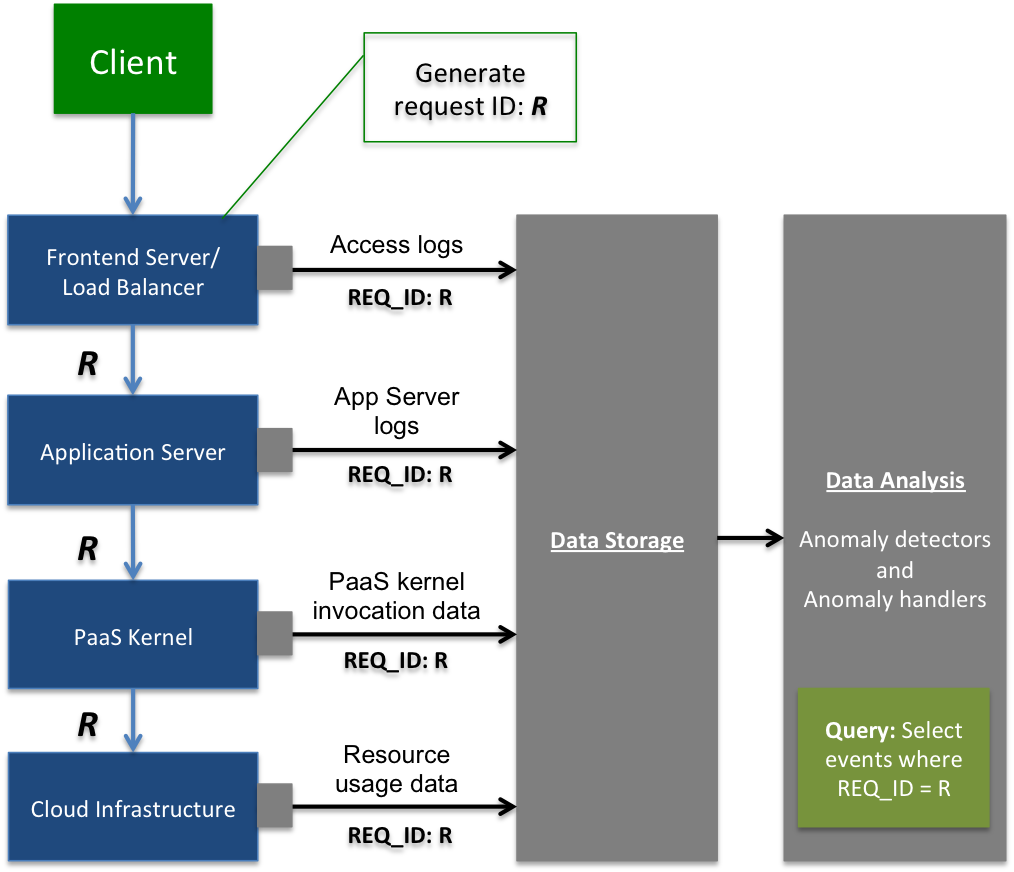
\includegraphics[scale=0.5]{apm_architecture}
\caption{Roots APM architecture.  Roots injects a request ID ($R$) at request
ingress that it uses to correlate events at each level of the stack.}
\label{fig:apm_architecture}
\end{figure}
%
%Figure~\ref{fig:apm_architecture} illustrates the high-level architecture of Roots, and how 
%it fits into the PaaS stack. APM components are shown in grey, with their interactions indicated
%by the black lines. The small grey boxes attached to the PaaS components represent the
%agents used to instrument the cloud platform for data collection purposes. 
%In the diagram a user request is getting tagged with the identifier value
%$R$ at the front-end server. This identifier is passed down to the lower layers of the cloud
%along with the request. Events that occur in the lower layers as a result of processing this request
%are recorded with the request identifier $R$, so we can correlate them later. For example, in the 
%data analysis component we can run a filter query to select all the events related to a particular
%request (as shown in the pseudo query in the diagram). Or we can run a ``group by'' 
%query to select all events, and aggregate them by the request identifier.

Figure~\ref{fig:apm_architecture} shows Roots collecting data from all
layers in a PaaS stack (i.e. full stack monitoring). 
%From the front-end server layer we gather information related to incoming application
%requests. A big part of this is scraping the HTTP server access logs, which indicate request timestamps,
%source and destination addressing information, response time (latency) and other HTTP message
%parameters. This information is readily available for harvesting in most technologies used as front-end
%servers (e.g. Apache HTTPD, Nginx). Additionally we may also collect information pertaining to active
%connections, invalid access attempts and other errors.
%
%From the application server layer we collect basic application logs as well as any other
%metrics that can be easily collected from the application runtime. This may include some process level
%metrics indicating the resource usage of the individual application instances. Additionally, Roots
%employs a set of per-application benchmarking processes that periodically probes 
%different applications
%to measure their performance. These are lightweight, stateless processes managed by the Roots framework.
%Data collected by these processes will also be sent to data storage component, and will be available
%for analysis as per-application time series data. 
%
%In particular, for each request 
%at the PaaS kernel layer we collect information regarding all kernel invocations
%made by the applications. This requires intercepting the PaaS kernel invocations
%at runtime. This must be done carefully as to not introduce a noticeable
%overhead to the application execution. For each PaaS kernel invocation, 
%we can capture the 
%following parameters.
%\begin{itemize}
%\item Source application making the kernel invocation
%\item Timestamp
%\item A sequence number indicating the order of PaaS kernel invocations within an application request
%\item Target kernel service and operation
%\item Execution time of the invocation
%\item Request size, hash and other parameters
%\end{itemize}
Collecting this information along with the request identifiers generated by the
front-end server
enables tracing the execution of application requests through the cloud platform. In addition
to the data collecting agents directly integrated with the cloud platform, Roots employs
a collection of application benchmarking processes that periodically measures
application latency. The measurements taken by these processes are mainly used to
evaluate the performance SLOs of each application.

%Finally, at the lowest infrastructure level, we can collect information related to virtual machines, containers
%and their resource usage. We can also gather metrics on network usage by individual components which
%might be useful in a number of traffic engineering use cases. Where appropriate we can also scrape
%hypervisor and container manager logs to get an idea of how resources are allocated and released over
%time.

To avoid introducing delays to the application request processing flow, we implement
all Roots data collecting agents as asynchronous tasks. That is, none of them would
suspend application request processing to report data to the data storage components.
We make sure that all expensive I/O tasks related to data collection and storage are
executed out of the request processing flow.
In particular, all data is collected into log files or memory buffers that are local to the components being
monitored. This locally collected (or buffered) data is periodically sent
to the data storage components of Roots using separate background tasks and batch communication
operations. Also special care is taken to isolate the activities in the cloud from potential
failures in the Roots data collection or storage components.

\subsubsection{Data Storage}

The Roots data storage is a database that supports persistently storing monitoring data, and running
queries on them.  
%Cloud providers have the freedom to implement this component in any way they see fit, as long
%as it scales to the number of applications deployed in the cloud platform. 
Most data retrieval queries executed
by Roots use application and time intervals as indices. Therefore a database that can index monitoring
data by application, and then organize records by timestamp will greatly improve the query performance.
It is also acceptable to remove old monitoring data to make room for more recent events, since Roots
is performing anomaly detection using the most recent data in near real time.

\subsubsection{Data Analysis}

Roots data analysis component uses two basic abstractions: \textit{anomaly detectors} 
and \textit{anomaly handlers}.
Anomaly detectors are processes that periodically analyze the data collected for
each deployed application. Roots supports multiple detector implementations, where each implementation
uses a different statistical method to look for performance anomalies. Detectors are configured
per-application, making it possible for different applications to use different anomaly 
detectors. Roots also supports multiple concurrent anomaly detectors on the same application, which can be used
to evaluate the efficiency of different detection strategies for any given application. Each
anomaly detector has an execution schedule (e.g. run every 60 seconds), and a sliding window 
(e.g. from 10 minutes ago to now)
associated with it. The boundaries of the window determines the time range
of the data processed by the detector at any round of execution. Window is updated 
after each round of execution. 
%Our anomaly detector abstraction is general
%enough to support detecting a wide range of anomalies. However, in our work we
%mainly focus on anomaly detectors that check for violations of performance SLOs.

When an anomaly detector finds an anomaly in application performance, it sends an event
to a collection of anomaly handlers. The event encapsulates a unique anomaly identifier, 
timestamp, application identifier and the source detector's sliding window that correspond to the
anomaly. Anomaly handlers are configured globally (i.e. each handler
receives events from all detectors), but each handler can be programmed to handle only
certain types of events. Furthermore, they can fire their own events, which are also delivered to
all the listening anomaly handlers. Similar to detectors, Roots supports multiple anomaly handler
implementations -- one for logging anomalies, one for sending alert emails, one
for updating a dashboard etc. 

Additionally, Roots includes two special anomaly handler
implementations: a workload change analyzer, and a bottleneck identifier.
The communication between detectors and handlers can be efficiently implemented
using shared memory as explained in section ~\ref{sec:process_mgt}.

%The ability of anomaly handlers to fire their own events, coupled with their support
%for responding to a filtered subset of incoming events enables constructing
%elaborate event flows with sophisticated logic. For example, the workload
%change analyzer can run some analysis upon receiving an anomaly event
%from any anomaly detector. If an anomaly cannot be associated with a workload
%change, it can fire a different type of event. The bottleneck identifier, can
%be programmed to only execute its analysis upon receiving this second type of event.
%This way we perform the workload change analysis first, and perform the
%systemwide bottleneck identification only when it is required to do so.

%Both the anomaly detectors and anomaly handlers work with fixed-sized sliding windows.
%They can discard any old data as the sliding window moves along the time line.
%Therefore the amount of state information these entities must keep in memory has
%a strict upper bound. 
%The extensibility of Roots is primarily achieved through the abstractions of anomaly
%detectors and handlers. Roots makes it simple to implement new detectors and handlers,
%and plug them into the system. Both the detectors and the handlers are executed
%as lightweight processes that do not interfere with the rest of the processes in
%the cloud platform. Failures in detectors and handlers have no impact
%on the cloud platform or the deployed applications.

\subsubsection{Roots Pods}
\label{sec:process_mgt}

%\begin{figure}
%\centering
%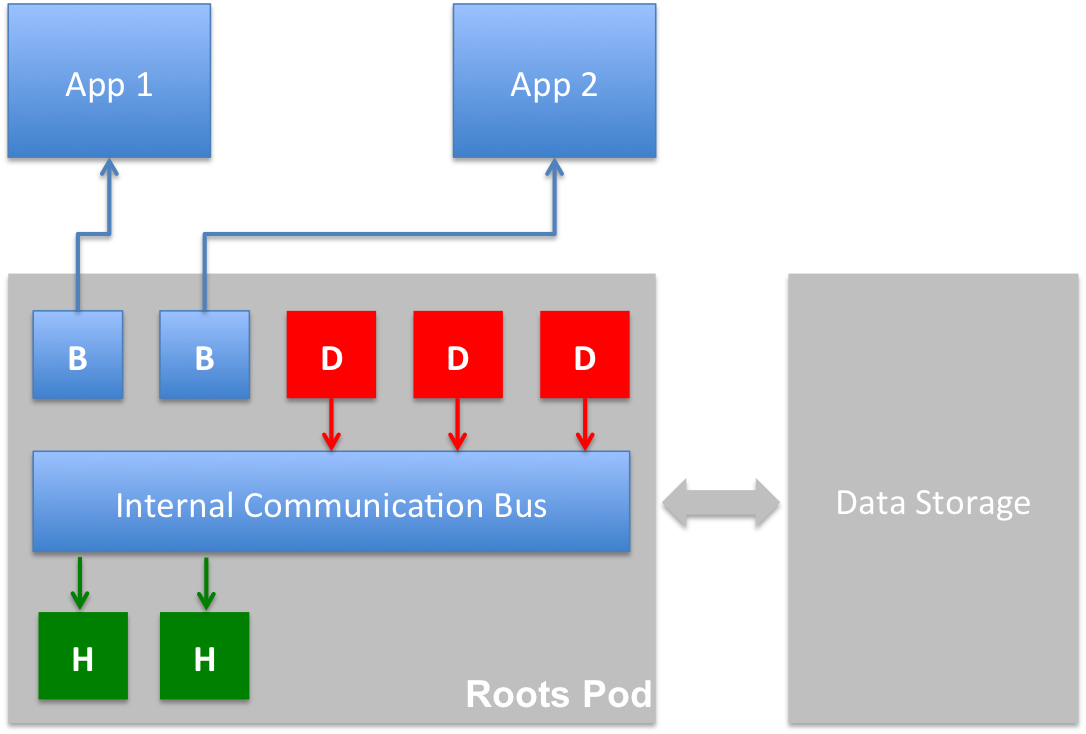
\includegraphics[scale=0.45]{roots_pod}
%\caption{Anatomy of a Roots pod. The diagram shows 2 application benchmarking processes (B), 
%3 anomaly detectors (D), and 2 handlers (H). Processes communicate via a shared
%memory communication bus local to the pod.}
%\label{fig:roots_pod}
%\end{figure}
%Most data collection activities in Roots can be treated as passive -- i.e. they
%happen automatically as the applications receive and process requests in the cloud
%platform. They do not require explicit scheduling or management. In contrast,
%application benchmarking and data analysis are active processes that require
%explicit scheduling and management.  This is achieved by 

Roots groups data analysis processes (i.e. anomaly detectors and handlers), 
and application benchmarking processes into units called \textit{Roots pods}. 
Each Roots pod is responsible for starting and maintaining a collection of
benchmarkers and data analysis processes. 
Each of these processes are light enough, so as to pack a large number of them
into a single pod. Pods are self-contained entities, and there is no inter-communication
between pods. 
Processes within a pod can efficiently communicate with each other 
using shared memory, and call out to the central Roots data storage to retrieve 
collected performance data for analysis. This enables starting and stopping 
Roots pods with minimal impact on the overall monitoring system. Furthermore, pods
can be replicated for high availability, and application load can be distributed
among multiple pods for scalability.

%Figure~\ref{fig:roots_pod} illustrates a Roots pod monitoring two applications.
%It consists of two benchmarking processes, three anomaly detectors and 
%two anomaly handlers. The anomaly detectors and handlers communicate
%using an internal shared memory communication bus, so that events triggered by one anomaly
%detector flow into all handlers. 

%To automate the process of managing pods, they can be tied into the core
%process management framework of the PaaS cloud. That way whenever the cloud
%platform initializes, a collection of pods can be started automatically.
%Application deployment process of the PaaS cloud can be augmented
%to register each new application with one of the available pods, so that the
%benchmarkers and anomaly detectors can start running on the application.
%Moreover, pods can be moved around or restarted as needed in response
%to errors and autoscaling events that occur in the cloud platform.


\section{Prototype Implementation}
\label{sec:impl}
To investigate the efficacy of Roots as an approach to
implementing performance diagnostics as a PaaS service, we have developed a
working prototype, and a set of algorithms that uses it to automatically
identify SLO-violating performance anomalies.
For this investigation, we integrate Roots into AppScale~\cite{6488671}, an open source PaaS cloud
that is API-compatible with the Google App Engine~\cite{gae} public cloud.  
AppScale can run on bare metal or within cloud infrastructures (Amazon EC2, Eucalyptus, 
etc.), and executes GAE applications without modification.
We minimally modify AppScale's internal components to integrate Roots.

\begin{figure}
\centering
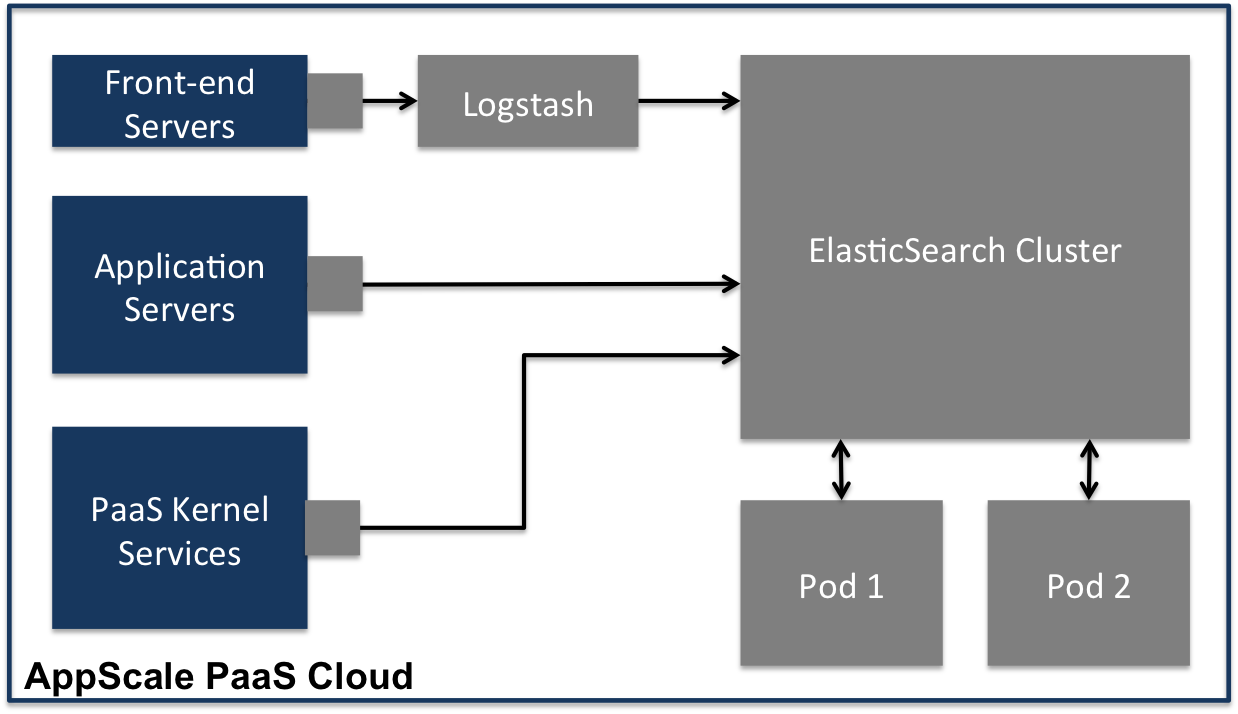
\includegraphics[scale=0.3]{roots_impl}
\caption{Roots prototype implementation for AppScale PaaS.}
\label{fig:roots_impl}
\end{figure}

Figure~\ref{fig:roots_impl} shows an overview of our prototype implementation. Roots components
are shown in grey, while the PaaS components are shown in blue.
We use ElasticSearch~\cite{Kononenko:2014:MMR:2597073.2597091} for data storage in our prototype. 
We configure AppScale's front-end server (Nginx) to tag all incoming application requests
with a unique identifier via a custom HTTP header. 
All data collecting agents in the cloud extract this identifier, and include it as an attribute
in all the events reported to ElasticSearch. This enables our prototype to aggregate events based 
on request IDs.

We implement a number of data collecting agents in AppScale to gather runtime information
from all major components of the PaaS. These agents buffer data locally, and store them in ElasticSearch
in batches. Roots persist events when the buffer accumulates 1MB of data or every 15 seconds, whichever comes
first.  This ensures that the events are promptly reported to the Roots data
storage while keeping the memory footprint of the data collecting agents small and bounded. 
For scraping server logs and storing the extracted entries in ElasticSearch,
our prototype uses Logstash~\cite{logstash}. 
To capture the PaaS kernel invocation data, we augment AppScale's PaaS kernel implementation,
which is derived from the GAE PaaS SDK. Specifically, we implement a Roots agent that monitors
and times all PaaS kernel invocations, and reports them to ElasticSearch. 

We implement Roots pods, which contain more computationally intensive Roots components, 
as standalone Java server processes. We use threads to run benchmarkers,
anomaly detectors, and handlers concurrently within each pod. Pods communicate with ElasticSearch via
a web API, and many of the data analysis tasks such as filtering and aggregation are performed
directly in ElasticSearch.

\subsection{Detecting SLO Violations}

The SLO-based anomaly detector of Roots
allows application developers to specify simple performance SLOs for deployed applications. A
performance SLO is an upper bound on the application response time ($T$), and a probability ($p$)
that the application response time is below the specified upper bound. 
When activated, the detector starts an application benchmarking process within a Roots pod
that periodically measures the response time of the target application. Probes made by the benchmarking 
process are several seconds apart in time (defined by the process sampling rate), 
so as not to degrade application performance.
The detector periodically
analyzes the collected response time measurements to check if the application meets the specified performance
SLO. The detector also accepts a minimum sample count as a parameter. This is the minimum number of 
samples the detector should take before evaluating an SLO.  If the fraction of response time measurements
that are
less than $T$ falls below $p$, the SLO has been violated, and Roots triggers an anomaly event.

To prevent the detector from detecting the same anomaly multiple times, we flush
the detection window upon each SLO violation. A side effect of this is that 
the detector is unable to detect
another violation until the window fills again.
For a sampling rate of 15 seconds and a minimum
sample count of 100, this ``warm up'' period will be 25 minutes.

%\subsection{Path Distribution Anomalies}
%%
%We have implemented a path distribution analyzer and anomaly
%detector in Roots. Its function is to identify recurring sequences of
%PaaS kernel invocations made by an application.
%Each identified sequence corresponds to a path of
%execution through the application code (i.e. a path through the control flow graph of the application). 
%This detector is able to determine the frequency with
%which each path is executed over time. Then, using this information which we term
%a ``path distribution,'' it reports an anomaly when the distribution of call paths
%changes. 
%
%%For each application,
%%a path distribution is comprised of the set of execution paths available in
%%that application, along with the proportion of requests that executed each path.
%%It is an indicator of the type of request workload handled by an application.
%%For example consider a data management application that has a read-only execution path, and a read-write 
%%execution path. If 90\% of the requests execute the read-only path, and the remaining 10\% of the requests
%%execute the read-write path, we may characterize the request workload as read-heavy.
%
%%
%%is another special anomaly detector we implement in Roots. This
%%anomaly detector periodically analyzes the PaaS kernel invocations made by the applications.
%By aggregating the PaaS kernel invocations by application request identifiers, and then sorting them by
%their sequence numbers, this anomaly detector is able to identify the sequence of
%PaaS kernel invocations made by each application request. 
%Each identified invocation sequence corresponds to a path of
%execution through the application code (i.e. a path through the control flow graph of the application). 
%Then the anomaly detector evaluates the number of requests
%that invoked the same PaaS kernel invocation sequence. From that the anomaly detector
%computes the distribution of different execution paths of an application.
 
%Roots path distribution analyzer facilitates computing the path distribution for each application
%with no static analysis, by only analyzing the runtime data gathered from the applications.
%The Roots path distribution analyzer  periodically computes the path distribution for a given application.
%If it detects that the latest path distribution is significantly different from the distributions seen in the 
%past, it triggers an anomaly. This is done by computing the mean request proportion for each path
%(over a sliding window of historical data),
%and then comparing the latest request proportion values against the means. If the latest proportion
%is off by more than $n$ standard deviations from its mean, the detector considers it to be an
%anomaly. The sensitivity of the detector can be configured by changing the value of $n$, which
%defaults to 2. 

%This anomaly detector enables developers to know when the nature of their application request
%workload changes. For example in the previous data management application, if suddenly 90\%
%of the requests start executing the read-write path, the Roots path distribution analyzer will
%detect the change as an anomaly. Similarly it is also able to detect when new paths of execution
%are being invoked by requests (a form of novelty detection).

\subsection{Workload Change Analyzer}

To detect changes in workload, Roots implements a workload change analyzer as an anomaly handler. 
This handler is invoked for every anomaly detected by Roots.
The workload change analyzer determines if an anomaly is due to a change in workload (i.e.
an increase in the application request rate). Roots can report
changes in workload via alerts; PaaS administrators can use such alerts to determine when to
add resources to the system.
Roots subjects anomalies \textit{that are not due to a workload change} to bottleneck
identification.

In contrast to the method described 
in~\cite{Magalhaes:2010:DPA:1906485.1906774,
Magalhaes:2011:RAP:1982185.1982234} which uses correlation between request
latency and workload, our 
workload change analyzer uses change point detection algorithms to identify changes in
the application's request rate. 
Our implementation of Roots supports a number of well known change point
detection algorithms (PELT~\cite{doi:10.1080/01621459.2012.737745}, binary segmentation 
and CL method~\cite{chen1993joint}), any of which can be used to detect level shifts in the
workload size.  For the results in this paper, we use PELT to detect changes in workload.
% Algorithms like PELT favor long lasting shifts (plateaus) in the workload trend, over momentary spikes.
%We expect momentary spikes to be fairly common in workload data. But it's the plateaus that cause
%request buffers to fill up, and consume server-side resources for extended periods of time, thus
%causing noticeable performance anomalies.

\subsection{Bottleneck Identification}

Roots performs bottleneck identification for any performance
anomalies that are triggered by something other than a change in workload.
To enable this, Roots performs multiple analyses over the PaaS performance data that it
collects using full-stack monitoring, without application instrumentation.

PaaS applications 
consist of user code that is executed in one or more application servers,
which makes remote service calls to PaaS kernel services. 
AppScale provides the same kernel services provided by GAE (datastore, memcache,
urlfetch, blobstore, user management etc.).
We consider each PaaS kernel invocation and the code running in the application server as 
separate \textit{components}. Each application request causes one or more components to
execute, and any one of the components can become a bottleneck to cause performance anomalies.  
The purpose of bottleneck identification is to find, across all
the components executed by an application, the one that is most likely to have 
degraded application performance.

Roots tracks the total time and the time spent in individual components for each request, 
and relates them via the formula $T_{total} = T_{X_1} + T_{X_2} + ... + T_{X_n} + r$. 
$T_{total}$ is the total execution time of a request. $T_{X_i}$ is the time spent executing
$X_i$; the $i^{th}$ PaaS kernel invocation.  $r$ is the time spent in the resident
application server executing user code (i.e. the time
spent not executing PaaS services during a request). Roots measures the $T$ values in the platform, and
computes $r$ using this formula. $r$ is not measured directly because doing so would require 
application instrumentation. Given that typical PaaS-hosted web
applications spend most of their time executing platform 
services~\cite{Jayathilaka:2015:RTS:2806777.2806842},
we expect $r \ll T_{X_1} + T_{X_2} + ... + T_{X_n}$ in the common case.

\subsubsection{Selecting Bottleneck Candidates}

Roots employs multiple candidate selection algorithms to identify up to four 
components that are potentially
the bottleneck responsible for the detected anomaly. Our algorithms look for
a variety of inconsistencies and changes in the performance characteristics of 
individual components.  In our prototype, we consider the relative importance of components, 
variations in relative importance, and two 
distributional techniques that distinguish rare events and 
outliers in performance history.

\paragraph*{Relative Importance}
Relative importance~\cite{JSSv017i01} identifies the component that is contributing 
the most towards the variance in the total response time. 
To use it, we regress the kernel calls against the total response time.
That is, for a time window $W$ just prior to the detection of the anomaly, Roots
fits a linear model using linear regression of the form
$T_{total} = T_{X_1} + T_{X_2} + ... + T_{X_n}$
over the per-request performance data in the window.

We omit $r$ since it is typically small.
For cases in which the anomaly occurs in $r$ (e.g. a performance problem in the 
application server or user code), $r$ may
not fit our assumption that $r \ll T_{X_1} + T_{X_2} + ... + T_{X_n}$.  When this
occurs, we assume that $r$ is normally distributed and independent, and filter out
requests from the window for which $r$ is larger than the 0.95 quantile ($r > \mu_r + 1.65\sigma_r$)
to preclude them from skewing the regression. 
We consider the influence of $r$ in other methods described below.

Roots ranks the regressors (i.e. $T_{X_n}$ values) based on their contribution to the variance 
in $T_{total}$.  We use the LMG method~\cite{lmg80} to do so which is resistant to multicollinearity, 
and provides a breakdown of the $R^2$ value of
the regression according to how strongly each regressor influences
the variance of the dependent variable ($T_{total}$).
Roots selects the highest ranked component as a candidate.

\paragraph*{Change in Relative Importance}
The next method selects the most likely candidate by detecting \textit{changes} in relative importance
over time.
This indicates how the variance a component contributes towards the total response time has
changed over time.
For this method, Roots divides the time window $W$ into equal-sized segments,
and computes relative importance for regressors within each segment. 
This results in multiple time series of relative importance values.
We subject each relative importance time series to change point analysis (PELT in our prototype), 
and extract the variable that shows an increase in relative importance, if any.
If such a variable is found, then the component
associated with that variable is considered by Roots as a bottleneck candidate.
The candidate selected by this method represents
a component whose performance has been stable in the past, and has become variable recently.

\paragraph*{High Quantiles}
Next we turn our attention to the distributions of $T_{X_k}$ and $r$.
Out of all the available distributions,
we wish to find the one whose quantile values are the largest.
Specifically, we compute a high	
quantile (e.g. 0.99 quantile) for each distribution. The component, whose distribution
contains the largest quantile value
is chosen as another potential candidate for the bottleneck. This component can be considered
as having a high latency in general.

\paragraph*{Tail End Values}
Finally, Roots analyzes each $T_{X_k}$ and $r$ distribution to identify the one 
with the largest tail values with respect to a particular high quantile.
For each tail end value $t$, we compute the metric $P^q_t$. 
This is the percentage difference between $t$ and the
$q$ quantile of the corresponding distribution. We set $q$ to 0.99 in our experiments.
Roots selects the component with the 
distribution that has the largest $P^q_t$ as another potential bottleneck candidate.
This method identifies
candidates that contain rare, high-valued outliers (point anomalies) in their distributions.

\subsubsection{Selecting Among Candidates}
We use a simple scoring mechanism to identify the root cause of a bottleneck 
from the selected candidates. There are at most four candidates to consider.  
The method assigns 4 points to the component chosen
by relative importance, and 3 points to all other candidates. 
We declare the bottleneck component as the one with the largest
point sum.  This method uses relative importance as the tie-breaker because it
targets components with consistently high variance, and thus is able to identify
longer lasting performance issues in the system
(i.e. collective anomalies~\cite{Chandola:2009:ADS:1541880.1541882}).
Prior work~\cite{Magalhaes:2011:RAP:1982185.1982234} has shown that 
regression-based techniques are highly effective in root cause analysis.


\section{Results}
\label{sec:results}
We wish to understand the efficacy of Roots
in terms of its ability to identify and characterize SLO violations,
We also wish to understand how well it identifies the
bottleneck component when a violation is not caused by a workload change.
Finally, we wish to investigate the performance and scalability of the Roots
prototype. 
%\begin{itemize}
%\item its ability to identify SLO violations,
%\item its ability to characterizes each correctly-identified SLO violation as
%being due to a workload change or a bottleneck,
%\item when there is a bottleneck, its ability to identify the correct
%bottleneck, 
%\item the speed with which it reacts to anomalies, and
%\item its failure rate (accuracy).
%\end{itemize}
%%its ability to detect performance anomalies, and correctly
%%identify the component responsible for each anomaly.  
%Additionally, we wish
%to characterize the overhead introduced by Roots in terms of its effect on
%perceived application performance, and determine the degree to which Roots
%pods enable scalability.

\subsection{Roots Efficacy}

\begin{table}
{\footnotesize
\begin{center}
\begin{tabular}{|c|p{1cm}|p{1cm}|p{1cm}|}
\hline
Faulty Service & $L_1$ (30ms) & $L_2$ (35ms) & $L_3$ (45ms) \\ \hline
datastore & 18 & 11 & 10 \\ \hline
user management & 19 & 15 & 10 \\ \hline
\end{tabular}
\end{center}
}
\vspace{-0.2in}
\caption{\textit{Number of anomalies detected in guestbook app under different SLOs 
($L_1$, $L_2$ and $L_3$) when injecting faults into two different PaaS kernel services.
\label{tab:anomaly_counts}
}}
\vspace{-0.2in}
\end{table}

To begin the evaluation of the Roots prototype we experiment with
the SLO-based anomaly detector, using a simple HTML-producing Java 
web application called ``guestbook''.
This application allows users to login, and post comments. It uses the
AppScale  datastore service to save
the posted comments, and the AppScale user management service to handle authentication. Each request processed
by guestbook results in two PaaS kernel invocations -- one to check if the user is logged in, and 
another to retrieve the existing comments from the datastore. We conduct all
our experiments on a single node AppScale cloud except where specified. The node itself is an Ubuntu
14.04 VM with 4 virtual CPU cores (clocked at 2.4GHz) and 4GB of memory.

We run the SLO-based anomaly detector on guestbook with a sampling rate of 15 seconds, an analysis
rate of 60 seconds, and a window size of 1 hour. We set the minimum samples count to 100, and
run a series of experiments with different SLOs on the guestbook application. Specifically, we fix
the SLO success probability at 95\%, and set the response time upper bound to $\mu_g + n\sigma_g$. 
$\mu_g$ and $\sigma_g$ represent the mean and standard deviation of the
guestbook's response time. We learn these two parameters \textit{a priori} by benchmarking
the application. Then we obtain three different upper bound values for the guestbook's
response time by setting 
$n$ to 2, 3 and 5 and denote the resulting three SLOs $L_1$, $L_2$ and $L_3$ respectively.

We also inject performance faults into AppScale by modifying its code
to cause the datastore service to be slow to respond.
This fault injection logic activates once every hour, and
slows down all datastore invocations by 45ms over a period of 3 minutes.
We chose 45ms because it is equal 
to $\mu_g + 5\sigma_g$ for the AppScale deployment under test. 
Therefore this delay is sufficient to violate all three SLOs used in our experiments. 
We run a similar set of experiments where we inject faults into the user management service of
AppScale. Each experiment is run for a period of 10 hours.

\subsection{Anomaly Detection Accuracy}

Table~\ref{tab:anomaly_counts} shows how the number of anomalies detected by 
Roots in a 10 hour period varies when the SLO is changed. The number of anomalies
drops noticeably when the response time upper bound is increased. When the $L_3$
SLO (45ms) is used, the only anomalies detected are the ones
caused by our hourly fault injection mechanism. As the SLO is tightened by lowering the upper bound,
Roots detects additional anomalies. These additional anomalies
result from a combination of injected faults, and other naturally occurring faults
in the system. That is, Roots detected some naturally occurring
faults (temporary spikes in application latency), when a number of injected faults
were still in the sliding window of the anomaly detector. Together these two types of
faults caused SLO violations, usually several minutes after the fault injection period
has expired.  In each case, however, a manual inspection of the data reveals
that Roots identified \textit{all} of the faults (injected and natural) correctly,
missing none
subject to the tightness of the SLO.

\subsection{Anomaly Detection Speed}

\begin{figure}
\centering
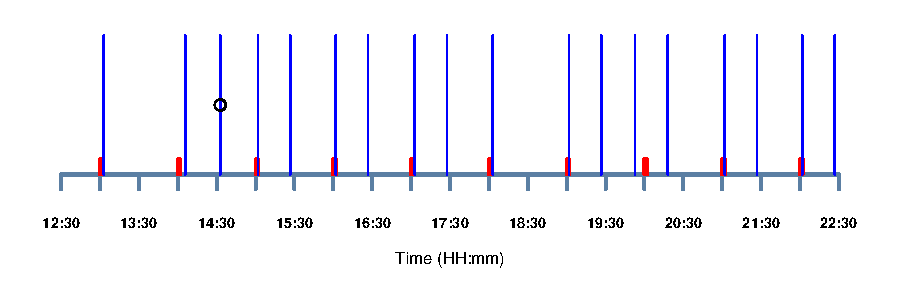
\includegraphics[scale=0.55]{time_line_guestbook_2s}
\vspace{-0.3in}
\caption{\textit{Anomaly detection in guestbook application during a period of 10 hours. Red arrows indicate fault injection
at the datastore service. Blue arrows indicate all anomalies detected by
Roots.
%during the experimental run.
}}
\label{fig:time_line_guestbook_2s}
\vspace{-0.2in}
\end{figure}

Next we analyze how fast and often Roots can detect anomalies in an application. We
first consider the performance of guestbook under the $L_1$ SLO while 
injecting faults into the datastore service. Figure~\ref{fig:time_line_guestbook_2s} shows
anomalies detected by Roots as events on a time line. The horizontal axis represents 
passage of time. The red arrows indicate the start of a fault injection period, where each
period lasts up to 3 minutes.
The blue arrows indicate the Roots anomaly detection events.
Note that every fault injection period is immediately followed by an anomaly
detection event, implying near real time reaction from Roots. The only exception is the fault
injection window at 20:00 hours which is not immediately followed by an anomaly 
detection event. Roots detected another naturally occurring anomaly
(i.e. one
that we did not explicitly inject but nonetheless caused an SLO violation) at 19:52 hours,
which caused the anomaly detector to go into the warm up mode. Therefore Roots
did not immediately react to the faults injected at 20:00 hours. But as soon as the detector became
active again at 20:17, it detected the anomaly.  Again, as in the previous
experiment, the detection accuracy was determined to be 100\% by manual
inspection.

%\begin{figure}
%\centering
%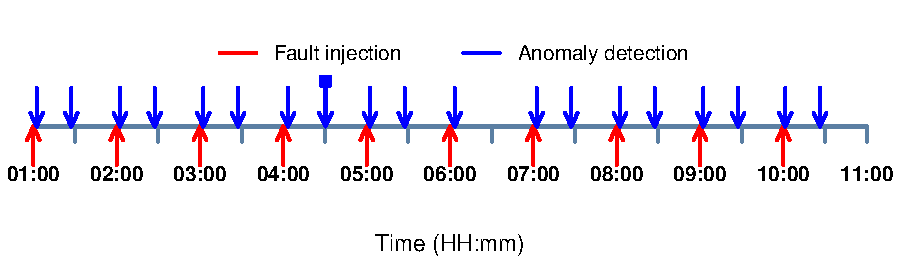
\includegraphics[scale=0.55]{time_line_guestbook_2s_user}
%\caption{Anomaly detection in guestbook application (timeline).}
%\label{fig:time_line_guestbook_2s_user}
%\end{figure}
%
%Figure~\ref{fig:time_line_guestbook_2s_user} shows the anomaly detection time line for the 
%same application and SLO, while faults are being injected into the user management service.
%Here too we see that Roots detects anomalies immediately following each fault injection window.

%\begin{figure}
%\centering
%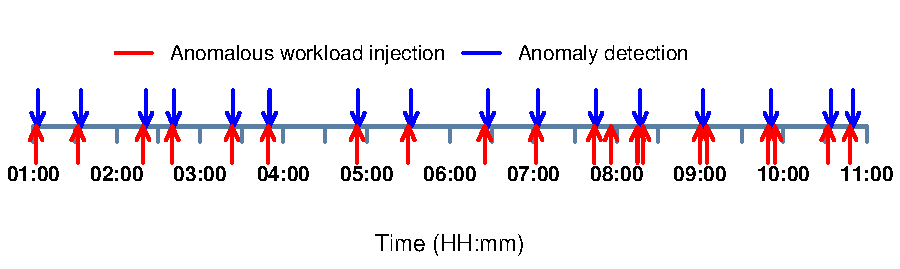
\includegraphics[scale=0.55]{time_line_crud}
%\caption{Path-distribution Anomaly detection in key-value store application (timeline). }
%\label{fig:time_line_crud}
%\end{figure}

%\begin{figure}
%\centering
%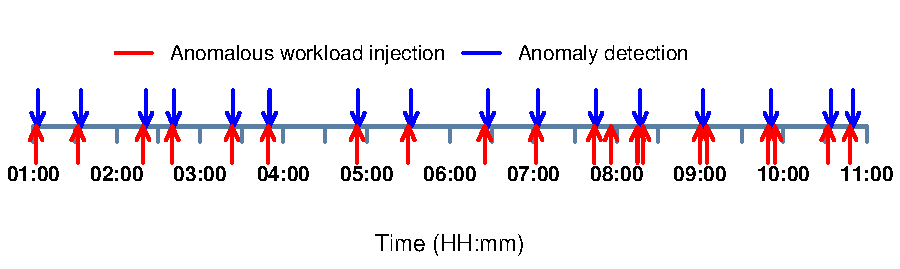
\includegraphics[scale=0.55]{time_line_caching}
%\caption{Anomaly detection in cached key-value store application (timeline).}
%\label{fig:time_line_caching}
%\end{figure}

%\subsection{Path Analyzer Accuracy and Speed}
%
%Next we evaluate the effectiveness and accuracy of the path distribution analyzer. For this we 
%employ a key-value store application. 
%%two different applications.
%%\begin{description}
%%\item[key-value store] 
%This application provides the functionality of an online key-value store.  It allows 
%users to store data objects in the cloud where each object is given a unique key. The objects can then be 
%retrieved, updated or deleted using their keys. Different operations
%(create, retrieve, update and delete) of the application are implemented as separate paths of
%execution in the application source code.
%%\item[cached key-value store] This is a simple extension of the regular key-value store, which adds
%%caching to the read operation using the AppScale's memcache service. The application contains
%%separate paths of execution for cache hits and cache misses.
%%\end{description}
%
%We first deploy the key-value store on AppScale, and populate it with a number of data objects. Then we
%run a test client against it which generates a read-heavy workload. On average this workload
%consists of 90\% read requests and 10\% write requests (create and update). The test client
%is also programmed to randomly send bursts of write-heavy workloads. These bursts consist
%of 90\% write requests on average, and each burst lasts up to 2 minutes. Figure~\ref{fig:time_line_crud}
%shows the write-heavy bursts as events on a time line (indicated by red arrows). Note that almost every burst is
%immediately followed by an anomaly detection event in Roots (indicated by blue arrows). The path
%distribution analyzer detects \textit{every} time the distribution of requests among different paths of execution
%changes significantly. The only time we do not see an anomaly detection event is when multiple
%bursts are clustered together in time (e.g. 3 bursts between 17:04 and 17:24 hours). In this
%case Roots detects the very first burst, and then goes into the warm up mode to collect more data. Therefore
%the bursts that immediately follow do not raise an alarm. These undetected
%events show the conditions under which Roots fails to detect anomalies.
%Events that occur while Roots is gathering a new sample after an anomaly is
%detected are missed.

%In addition,
%Between 20:30 and 21:00 hours we also
%had two instances where the read request proportion dropped from 90\% to 80\% due to random
%chance. This is because our test client randomizes the read request proportion around the 90\% mark. 
%In these two instances the read proportion was deemed too far off from 90\%, and Roots correctly 
%identified them as anomalies.

%We conduct a similar experiment using the cached key-value store. Here, we run a test client that generates a workload
%that is mostly served from the cache. This is done by repeatedly executing read requests on a small
%selected set of object keys. However, the client randomly sends bursts of traffic requesting keys that
%are not likely to be in the application cache, thus resulting in many cache misses. Each burst
%lasts up to 2 minutes. As shown in 
%figure~\ref{fig:time_line_caching}, Roots path distribution analyzer correctly detects the change 
%in the workload (from many cache hits to many cache misses), nearly every time the test client injects a 
%burst of traffic that triggers the cache miss path of the application. The only exception is when
%multiple bursts are clumped together, in which case only the first raises an alarm in Roots.

\subsection{Workload Change Analyzer Accuracy and Speed}

\begin{figure}
\centering
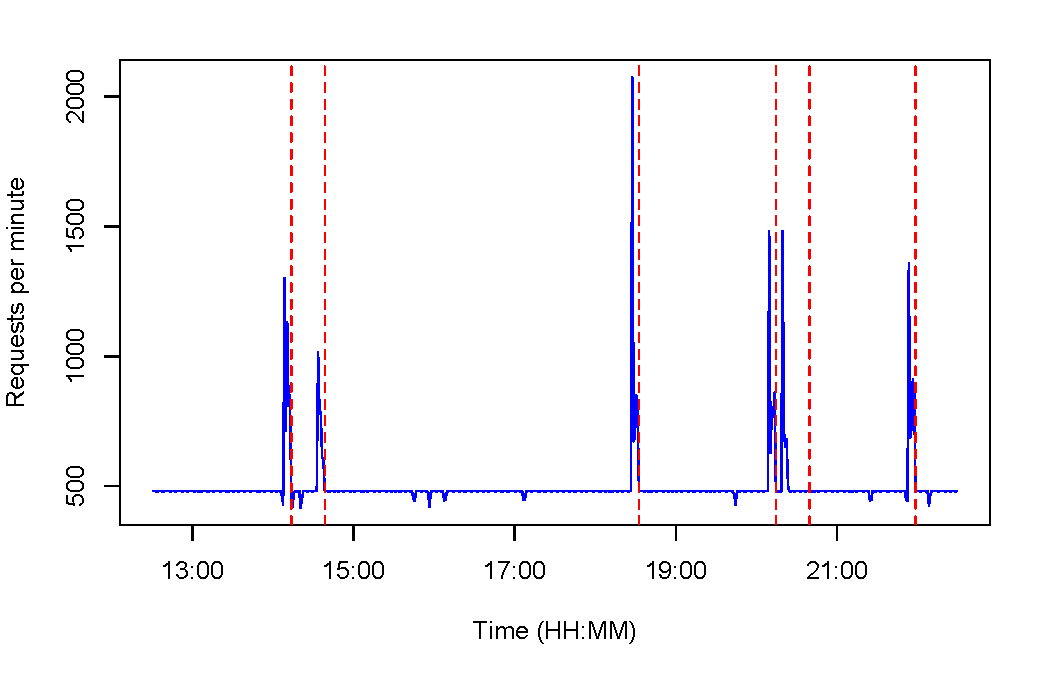
\includegraphics[scale=0.35]{workload_change_trace}
\vspace{-0.2in}
\caption{\textit{Workload size over time for the key-value store application. The test client randomly sends
large bursts of traffic causing the spikes in the plot. Roots anomaly detection events are shown
in red dashed lines.}}
\vspace{-0.2in}
\label{fig:workload_change}
\end{figure}

Next we evaluate the Roots workload change analyzer. In this experiment we run a varying workload
against a test application for 10 hours. The test application is an online key-value store that supports
basic data management operations. The load generating client is programmed
to maintain a mean workload level of 500 requests per minute. However, the client
is also programmed to randomly send large bursts of traffic at times of its choosing. During these bursts 
the client may send more than 1000 requests a minute, thus impacting the performance of
the application server that hosts the key-value store. Figure~\ref{fig:workload_change} shows how
the application workload has changed over time. The workload generator has produced 6 large bursts of traffic during the 
period of the experiment, which appear as tall spikes in the plot.
Note that each burst is immediately followed by a Roots anomaly detection event (shown by red dashed lines). 
In each of these 6 cases, the increase in workload caused a violation of the application performance SLO.
Roots detected the corresponding anomalies, and determined them to be caused by changes in the workload size.
As a result, bottleneck identification was not triggered for any of these anomalies.
Even though the bursts of traffic appear to be momentary
spikes, each burst lasts for 4 to 5 minutes thereby causing a lasting impact on the application performance.
The PELT change point detection method used in this experimental set up is ideally suited for detecting
such lasting changes in the workload level.

\subsection{Bottleneck Identification Accuracy}

Next we evaluate the bottleneck identification capability of Roots. We first discuss the results obtained using
the guestbook application, and follow with
results obtained using a more complex application.
In the experimental run illustrated in 
figure~\ref{fig:time_line_guestbook_2s}, Roots determined that all the detected anomalies except for one were 
caused by the AppScale datastore service. This is consistent with our expectations since in this experiment we 
artificially inject faults into the datastore. 
The only anomaly that is not traced back to the datastore service is the one that was detected at 14:32 hours.
This is indicated by the blue arrow with a small square marker at the top. For this anomaly, Roots concluded that
the bottleneck is the local execution at the application server ($r$). We have verified
this result by manually inspecting the AppScale logs and traces of data collected by Roots. As it turns out,
between 14:19 and
14:22 the application server hosting the guestbook application experienced some problems, which caused
request latency to increase significantly. Therefore we can conclude that Roots has correctly identified 
the root causes of all 18 anomalies in this experimental run
including one that we did not inject explicitly. 

%Similarly, in the experiment shown in figure~\ref{fig:time_line_guestbook_2s_user}, Roots determined
%that all the anomalies are caused by the user management service, except in one instance. This is again
%inline with our expectations since in this experiment we inject faults into the user management service. For the
%anomaly detected at 04:30 hours, Roots determined that local execution time is the primary bottleneck.
%In this case too the server hosting the guestbook application became slow
%during the 04:23 - 04:25 time window, and Roots correctly identified the bottleneck as the local
%application server.

\subsection{A More Complex Example}

\begin{figure}
\centering
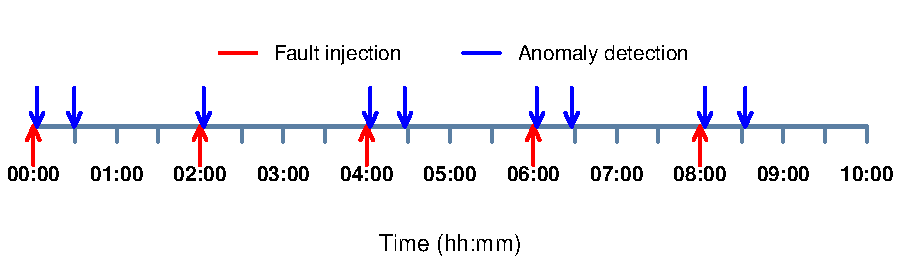
\includegraphics[scale=0.55]{time_line_stocks_1}
\vspace{-0.3in}
\caption{\textit{Anomaly detection in stock-trader application during a period of 10 hours. 
%Red arrows indicate fault injection
%at the 1st datastore query. Blue arrows indicate all anomalies detected by
%Roots during the experimental run.
}}
\vspace{-0.2in}
\label{fig:time_line_stocks_1}
\end{figure}

%\begin{figure}
%\centering
%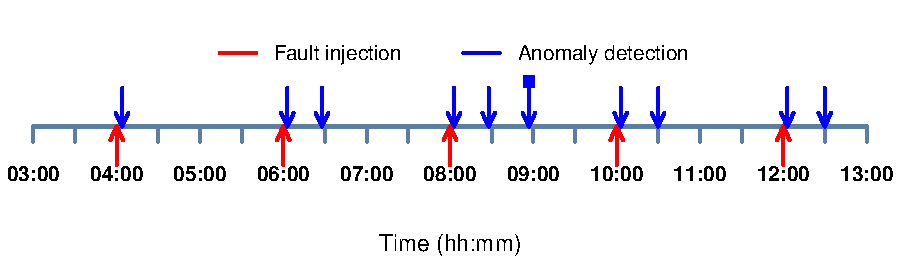
\includegraphics[scale=0.55]{time_line_stocks_2}
%\caption{Anomaly detection in stock-trader application (timeline).}
%\label{fig:time_line_stocks_2}
%\end{figure}

In order to evaluate how the bottleneck identification performs when an application makes more than 2
PaaS kernel invocations, we conduct another experiment using an application
called ``stock-trader''.
This application allows setting up organizations, and simulating trading of stocks between the
organizations. The two main operations in this application are \textit{buy} and \textit{sell}. Each of
these operations makes 8 calls to the AppScale datastore. 
According to our previous work~\cite{Jayathilaka:2015:RTS:2806777.2806842}, 8 kernel invocations in the
same path of execution is very rare in web applications developed for a PaaS cloud. The probability
of finding an execution path with more than 5 kernel invocations in a sample of PaaS-hosted
applications is less than 1\%. Therefore the stock-trader application is a good extreme case
example to test the Roots bottleneck identification support.
%We execute a number of experimental runs using this application,
%and here we present the results from two of them. 
In this experiment we configure the anomaly
detector to check for the response time SLO of 177ms with 95\% success probability.

In one of our experimental runs we inject faults into the first datastore query executed by the buy operation
of stock-trader. The fault injection logic runs every two hours, and lasts for 3 minutes. The duration of
the full experiment is 10 hours. 
Figure~\ref{fig:time_line_stocks_1} shows the resulting event sequence. Note that every fault injection
event is immediately followed by a Roots anomaly detection event. There are also four additional
anomalies in the time line which were SLO violations caused by a combination of injected faults, and
naturally occurring faults in the system. For all the anomalies detected
in this test, Roots correctly selected the first datastore call in the application code as the bottleneck. 
The additional four anomalies occurred because a large number of injected faults were in the sliding window
of the detector. Therefore, it is accurate to attribute those anomalies also to the first datastore query
of the application.

%Figure~\ref{fig:time_line_stocks_2} shows the results from a similar experiment where we inject
%faults into the second datastore query executed by the operation. Here also Roots detects all the
%artificially induced anomalies along with a few extras. All the anomalies, except for one, 
%are determined to be caused by the second
%datastore query of the buy operation. The anomaly detected at 08:56 (marked with a square on top of the blue arrow) 
%is attributed to the fourth datastore query executed by the application. We have manually verified this
%conclusion to be accurate. Since 08:27 (when the previous anomaly was detected), the fourth datastore
%query has frequently taken a long time to execute (again, on
%its own), which resulted in an SLO violation at 08:56 hours.

%In the experiments illustrated in figures~\ref{fig:time_line_guestbook_2s}, 
%\ref{fig:time_line_guestbook_2s_user}, 
%and \ref{fig:time_line_stocks_1} 
%and \ref{fig:time_line_stocks_2} 
%we maintain
%the application request rate steady throughout the 10 hour periods. Therefore as expected,
%the workload change analyzer of Roots did not detect any significant shifts in the workload level. 
%Consequently, none of the anomalies detected in these 4 experiments were attributed to a workload change.
%The bottleneck identification was therefore triggered for each anomaly, always resulting in a performance diagnosis
%involving an application component.

%\begin{figure}
%\centering
%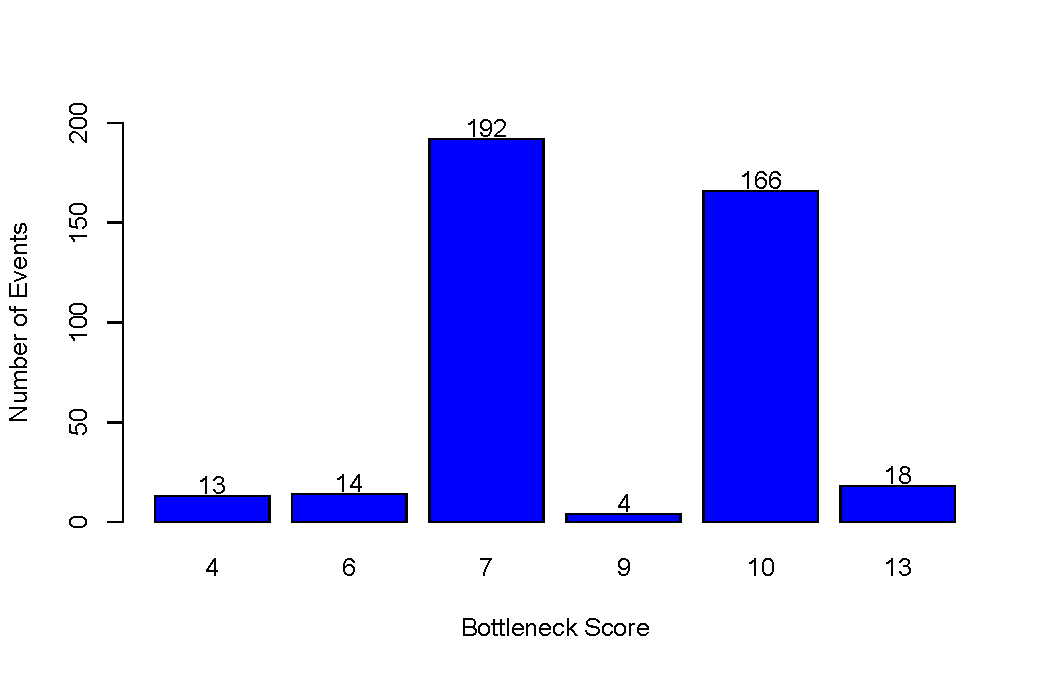
\includegraphics[scale=0.5]{bottleneck_scores}
%\caption{Frequency of different bottleneck scores.}
%\label{fig:bottleneck_scores}
%\end{figure}

%Recall that the bottleneck identification algorithm in Roots
%selects up to four candidate components for each performance anomaly detected, and then ranks them
%by assigning scores to identify the most likely bottleneck. Figure~\ref{fig:bottleneck_scores} shows the breakdown of 407 anomalies
%detected over a period of 3 weeks. X-axis represents the different scores given to candidate components
%by our algorithm. Y-axis shows the number of times a particular score was the highest. 
%According to this result, on 13 occasions Roots determined the bottleneck based on the highest score
%of 4 (score given to the component identified by the relative importance metric). 
%This happens when the algorithm chooses four different candidates
%for the bottleneck. However, this constitutes only 3.2\% of all the anomalies. In 96.8\% of the time Roots saw
%at least two of the four candidates to be the same (score values 6 or higher). This implies that most of the time Roots is able to
%identify bottlenecks with a high level of confidence since two or more candidate detection methods
%agree on their results.

\subsection{Multiple Applications in a Clustered Setting}

\begin{figure}
\centering
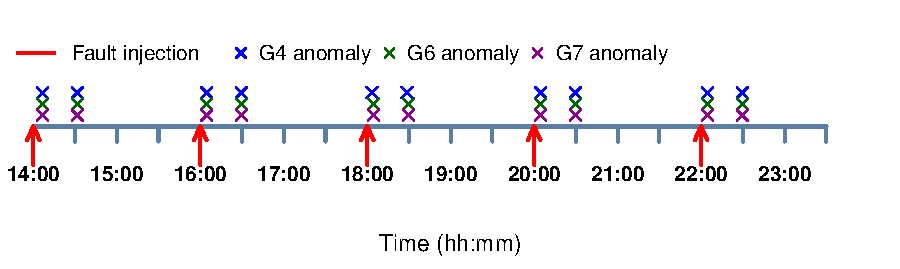
\includegraphics[scale=0.55]{time_line_g1g8}
\vspace{-0.3in}
\caption{\textit{SLO-violation Anomaly detection in 8 applications deployed in
a clustered AppScale cloud.}}
\vspace{-0.2in}
\label{fig:time_line_g1g8}
\end{figure}

So far we have been experimenting with a simple AppScale cloud deployed on a single virtual machine.
To demonstrate how Roots can be used in a multi-node environment, we set up an AppScale cloud
on a cluster of 10 virtual machines (VMs). VMs are provisioned by a
Eucalyptus~\cite{eucalyptus09} (IaaS)
cloud, and each VM is comprised of 2 CPU cores and 2GB memory. Then we proceed
to deploy 8 instances of the guestbook application on AppScale. We use the multitenant support
in AppScale to register each instance of guestbook as a different application ($G1$ through $G8$). This means each instance
is hosted on a separate application server instance, and has its own private namespace on the AppScale
datastore. Each application instance can be accessed via its own public URL. We disable auto-scaling support in 
the AppScale cloud, and inject faults into the datastore service of AppScale in such a way that queries
issued from a particular VM, are processed with a 100ms delay. We identify the VM by its IP address
in our test environment, and shall refer to it as $V_f$ in the discussion. We trigger
the fault injection every 2 hours, and when activated it lasts for up to 5 minutes. Then we monitor
the applications using Roots for a period of 10 hours. Each anomaly detector is configured
to check for the 75ms response time SLO with 95\% success rate. 
ElasticSearch, Logstash and the Roots pod are deployed on a separate VM. 

Figure~\ref{fig:time_line_g1g8} shows the resulting event sequence. Note that we detect anomalies 
in 3 applications ($G4$, $G6$ and $G7$) immediately after each fault injection. Inspecting the 
topology of our AppScale cluster revealed that these were the only 3 applications that were 
hosted on $V_f$. As a result, our bi-hourly fault injection caused their SLOs to
get violated. Other applications did not exhibit any SLO violations since we are monitoring against
a very high response time upper bound. In each case Roots detected the SLO violations 2-3 minutes into the fault injection
period. As soon as that happened, the anomaly detectors of $G4$, $G6$ and $G7$ entered the warmup mode.
But our fault injection logic kept injecting faults for at least 2 more minutes. Therefore when the anomaly detectors
reactivated after 25 minutes (time to collect the minimum sample count), they each saw another SLO
violation. This is why we see another set of detection events approximately half an hour after the
original fault injection events.

\subsection{Summarizing the Results}

Table~\ref{tab:results_summary} provides an overview of the efficacy
evalution.
\begin{table}
{\footnotesize
\begin{center}
\begin{tabular}{|p{2cm}|p{6cm}|}
\hline
Feature & Results Observed in Roots \\ \hline
Detecting accuracy &
The first occurance of all artificially induced anomalies were detected.
Roots also detected several ``natural'' anomalies in AppScale. \\ \hline
Anomaly Differentiation &
All anomalies were correctly identified as either due to workload change or
bottleneck. \\ \hline
Bottleneck Identification &
In all the cases where a bottleneck was identified Roots identified the
correct bottleneck. \\ \hline
Reaction time &
All induced SLO violations were detected as soon
as enough samples of the fault
were taken by the benchmarking process. \\
\hline
\end{tabular}
\end{center}
}
\vspace{-0.2in}
\caption{\textit{Summary of Roots efficacy results.
\label{tab:results_summary}
}}
\vspace{-0.1in}
\end{table}
While not exhaustive, these results indicate that Roots is able to achieve a
high degree of accuracy in detecting and characterizing performance anomalies
and then identifying the component or reason for each anomaly in a working,
production-quality open source PaaS.

\subsection{Roots Performance and Scalability}

Next we evaluate the performance overhead incurred by Roots on the applications deployed in the 
cloud platform. We are particularly interested in understanding the overhead of recording the PaaS kernel
invocations made by each application, since this feature requires some changes to the PaaS kernel
implementation. 
We deploy a number of applications on a vanilla
AppScale cloud (with no Roots), and measure their request latencies. We use
the popular Apache Bench tool to measure the request latency under a
varying number of concurrent clients. We then take the same measurements
on an AppScale cloud with Roots, and compare the results against the ones obtained
from the vanilla AppScale cloud. In both environments we disable the auto-scaling
support of AppScale, so that all client requests are served from a single application
server instance. In our prototype implementation of Roots, the kernel invocation events get buffered in
the application server before they are sent to the Roots data storage. We wish to
explore how this feature performs when the application server is under heavy load.

\begin{table}
{\footnotesize
\begin{center}
\begin{tabular}{|c|p{0.8cm}|p{0.8cm}|p{0.8cm}|p{0.8cm}|}
\hline &
      \multicolumn{2}{c|}{Without Roots} &
      \multicolumn{2}{c|}{With Roots} \\ \hline
    App./Concurrency & Mean (ms) & SD & Mean (ms) & SD\\

\hline
%guestbook/1 & 12 & 3.9 & 12 & 3.7 \\ \hline
guestbook/50 & 375 & 51.4 & 374 & 53 \\ \hline
%stock-trader/1 & 151 & 13 & 145 & 13.7 \\ \hline
stock-trader/50 & 3631 & 690.8 & 3552 & 667.7 \\ \hline
%kv store/1 & 7 & 1.5 & 8 & 2.2 \\ \hline
kv store/50 & 169 & 26.7  & 150 & 25.4  \\ \hline
%cached kv store/1 & 3 & 2.8 & 2 & 3.3 \\ \hline
%cached kv store/50 & 101 & 24.8 & 97 & 35.1  \\ \hline
\end{tabular}
\end{center}
}
\vspace{-0.2in}
\caption{\textit{Latency comparison of applications when running on
a vanilla AppScale cloud vs when running on a Roots-enabled
AppScale cloud.}
\label{tab:perf_overhead}
}
\vspace{-0.2in}
\end{table}

Table~\ref{tab:perf_overhead} shows the comparison of request 
latencies with 50 clients for each of the applications. 
We discover that Roots does not add a significant overhead
to the request latency in any of the scenarios considered. In all the cases,
the mean request latency when Roots is in use, is within one standard deviation
from the mean request latency when Roots is not in use. Also in a number
of cases the mean request latency is slightly lower when Roots is in use.

%The request latency increases when the number of concurrent clients is
%increased from 1 to 50 (since all requests are handled by a single
%application server), but still there is no sign of any detrimental overhead
%from Roots even under load. Since we buffer PaaS kernel invocation
%events in memory, and report them to ElasticSearch asynchronously, and
%out of the request processing flow, there is no measurable impact on
%the request latency from Roots.

%\begin{figure}
%\centering
%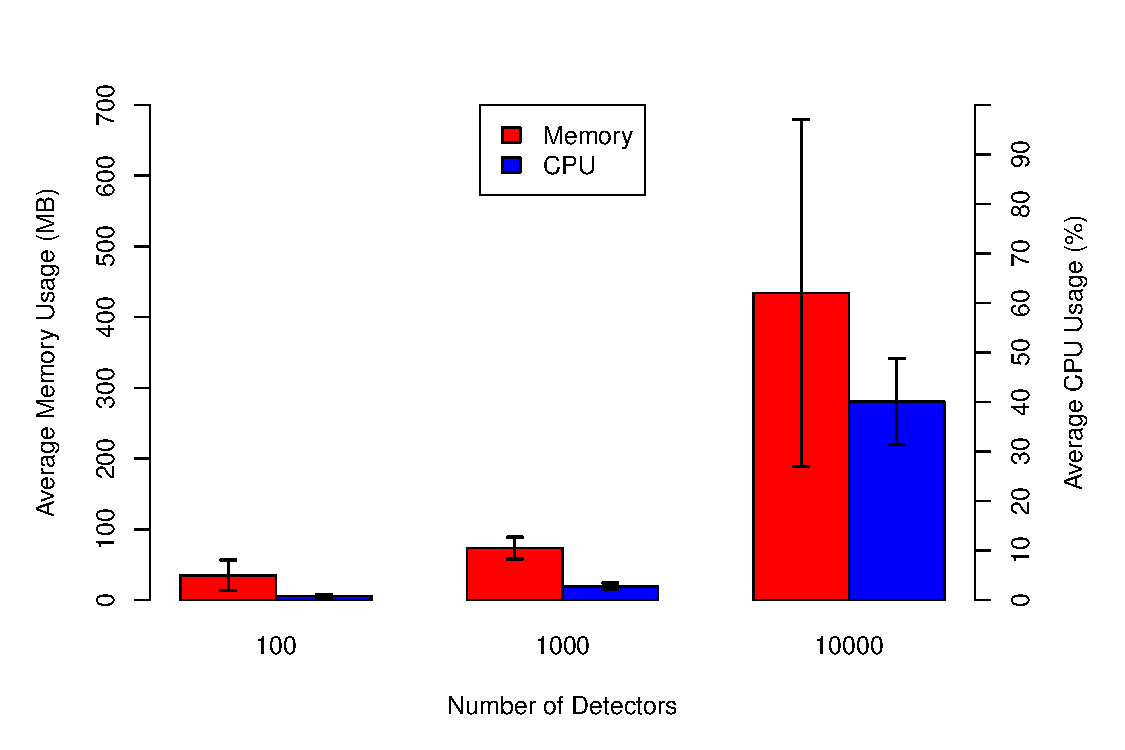
\includegraphics[scale=0.3]{pod_performance}
%\caption{Resource utilization of a Roots pod.}
%\label{fig:pod_performance}
%\end{figure}

Finally, to demonstrate Roots scalability, we deploy
a Roots pod on a virtual machine with 4 CPU cores and 4GB memory.
%
%To simulate monitoring multiple applications, we run multiple concurrent anomaly
%detectors in the pod. Each detector is configured with a 1 hour sliding window.
%We vary the number of concurrent
%detectors between 100 and 10000, and run each configuration for
%2 hours. We track the memory and CPU usage of the
%pod during each of these runs using the jstat and pidstat tools. 
%
%Figure~\ref{fig:pod_performance}
%illustrates the maximum resource utilization of the Roots pod for different counts of
%concurrent anomaly detectors. 
%
With 10000 concurrent detectors, the maximum memory usage of the pod was 778MB and the CPU usage
was 60\% of a single core.  Using just the one machine, with 4 cores and 4GB of
memory, a single pod was able to service 40000 concurrent detectors. 
Since one pod can service a large number of applications simultaneously
 and pods are independent, these results indicate that it is possible to scale Roots effectively.

%maximum CPU usage is 238\%, where 400\% is the available limit
%for 4 CPU cores. The maximum memory usage in this case is only 778 MB. 
%Since each anomaly detector operates with a fixed-sized window, and they
%bring additional data into memory only when required, the memory
%usage of the Roots pod generally stays low. In particular, the average resource usage
%is far less than the maximum usage values shown in figure~\ref{fig:pod_performance}. 
%For example, in case of 10000 detectors, the average CPU usage is only 32\%, and 
%the average memory usage is 507 MB. We also experimented with larger concurrent
%detector counts, and we were able to pack up to 40000 detectors into the pod before
%getting constrained by the CPU capacity of our quad-core VM.
%This result implies that we can monitor tens of thousands 
%of applications using a single pod, thereby scaling up to a very large number
%of applications using only a handful of pods.
%


\section{Related Work}
\label{sec:related_work}
Roots falls into the category of performance anomaly detection and bottleneck identification 
(PADBI) systems~\cite{Ibidunmoye:2015:PAD:2808687.2791120}. 
Such systems play a crucial role in achieving guaranteed performance and
quality of service by detecting performance issues in a timely manner before they escalate into major outages
or SLO violations~\cite{6045942}. 
However, the paradigm of cloud computing is yet to be
fully penetrated by PADBI systems research. The size, complexity and the dynamic nature of 
cloud platforms make performance monitoring a particularly challenging problem.
The existing technologies like Amazon CloudWatch~\cite{cloudwatch},
New Relic~\cite{newrelic} and DataDog~\cite{datadog} facilitate monitoring cloud applications 
by instrumenting low level cloud resources (e.g. virtual machines), and application code. But such technologies
are either impracticable or insufficient in
PaaS clouds where the low level cloud resources are hidden by abstractions.

Our work is heavily inspired by the past literature that detail the key features of 
cloud APMs~\cite{DaCunhaRodrigues:2016:MCC:2851613.2851619,Ibidunmoye:2015:PAD:2808687.2791120} . 
We also borrow from
Magalhaes and Silva who uses statistical correlation and linear regression to perform
root cause analysis in web applications~\cite{Magalhaes:2010:DPA:1906485.1906774, Magalhaes:2011:RAP:1982185.1982234}. 
Dean et al implemented PerfCompass~\cite{Dean:2014:PTR:2696535.2696551}, 
an anomaly detection and localization method for IaaS clouds. They instrument operating system kernels
of VMs to perform root cause analysis in IaaS clouds. We take a similar approach where we instrument
the kernel services of the PaaS cloud.
Nguyen et al presented PAL, another anomaly detection mechanism targeting
distributed applications deployed on IaaS clouds~\cite{Nguyen:2011:PPR:2038633.2038634}. 
Similar to Roots, they also use an SLO monitoring approach to detect anomalies.

\section{Conclusions}
\label{sec:conclusion}
We propose Roots, a near real time monitoring and diagnostics
framework for web applications and services deployed using a PaaS cloud. 
Roots is designed to function as a curated service
built into the cloud platform, as opposed to an external monitoring system. 
It relieves the application developers from having to configure
their own monitoring solutions or, indeed,
from having to instrument the application code.
%Roots captures runtime data from the different layers involved
%in processing application requests. It can correlate events across different layers
%to track the propagation of application requests through the cloud platform, and
%identify bottlenecks deep within the kernel services of the PaaS.

%Roots monitors applications for SLO compliance, and detects anomalies via SLO violations.
%When Roots detects an anomaly, 
%it analyzes workload data and other application runtime data
%to perform root cause analysis. Roots is able to determine whether a particular
%anomaly was caused by a change in the application workload, or due to a bottleneck
%in the cloud platform. To this end we also devise a bottleneck identification algorithm, that
%uses a combination of linear regression, quantile analysis and change point detection.

We evaluate Roots using a prototype built for the AppScale open source PaaS. 
Our results indicate that Roots is effective at detecting performance anomalies
in near real time. We also show that our bottleneck identification algorithm
produces accurate results nearly 100\% of the time (cf
Table~\ref{tab:results_summary}), pinpointing the exact PaaS
service or the application component responsible for each anomaly. Our empirical trials further 
reveal that Roots does not add a significant overhead to the applications deployed
on the cloud platform. Finally, we show that Roots is lightweight, 
and scales well to handle large populations of applications. 
%Specifically,
%we see that a single Roots pod is able to monitor tens of thousands of applications.

%In our future work we plan to expand the data gathering capabilities of Roots into
%the low level virtual machines and containers that host various services of the cloud
%platform. We intend to tap into the hypervisors
%and container managers to harvest runtime data regarding the resource usage (CPU, memory, disk etc.) of
%PaaS services and other application components. With that we expect to extend
%the root cause analysis support of Roots so that it can not only pinpoint the
%bottlenecked application components, but also the low level hosts and system
%resources that constitute each bottleneck.

\vspace{0.1in}
\noindent
This work is supported in part by NSF (CCF-1539586, CNS-0905237) and Huawei.


%\section{Related Work}
%Our research builds upon advances in the areas of SOA governance and
service management. 
Guan et al introduced FASWSM~\cite{1607141} a web service management
framework for application servers. Wu et al introduced DART-Man~\cite{1504267} a web
service management system based on semantic web concepts. 
Our work is different from these past approaches and 
from recent API management solutions~\cite{wso2am,apigee}
in that EAGER targets policy \textit{enforcement} 
and we focus on doing so by extending extant
cloud platforms to provide an integrated and scalable governance
solution.

Lin et al proposed a service management system for clouds that monitors all
service interactions via special ``hooks'' that are connected to the
cloud-hosted services~\cite{5616981}. However, this system only supports run-time
service management and provides no support for deployment-time governance. 
Kikuchi and Aoki~\cite{6525502} proposed a technique
based on model checking to evaluate the operational vulnerabilities and fault
propagation patterns in cloud services. But this system provides no
active monitoring or enforcement functionality.

Other researchers have shown that policies can be
used to perform a wide range of governance tasks for SOA such as access
control~\cite{4279630}, fault diagnosis~\cite{6154236},
and management~\cite{Suleiman:2009:IUM:1564601.1564730}. We build
upon these past efforts and use policies to govern
RESTful web APIs deployed in cloud settings. 
Peng, Lui and Chen showed that
the major concerns associated with SOA governance 
involve retaining the high reliability of services, recording how many services
are available on the platform to serve, and making sure all the available 
services are operating within an acceptable service
level~\cite{4730489}. EAGER attempts to satisfy similar requirements for 
modern RESTful web APIs deployed in cloud environments. 
However, EAGER's Metadata Manager and ADP record and keep track of all deployed APIs 
in a comprehensive manner.  Moreover, EAGER's governance features 
``fail fast'' to detect violations immediately.

%API management has been a popular topic in industry recently, resulting
%in many API management solutions~\cite{wso2am,apigee}. These products facilitate
%API lifecycle management, traffic shaping, access control, monitoring and a variety of other
%important API-related functionality. However, these tools do not support deep integration with
%cloud environments in which many web applications and APIs are deployed.

%
%These API
%management products either run as stand-alone entities or are layered on top of existing clouds
%thus leading to many maintenance, reliability and integration issues. Also, the support provided by these
%tools to specify and enforce policies in a flexible manner is very limited. EAGER is complementary
%to such tools, providing very deep integration with PaaS clouds thereby facilitating API governance
%as a core cloud-native feature. Indeed, EAGER can embed and enhance some of these tools to
%obtain the required API governance support in the cloud. In fact, the EAGER prototype we have
%implemented makes extensive use of an existing open source API management product~\cite{wso2am}.


%
% The following two commands are all you need in the
% initial runs of your .tex file to
% produce the bibliography for the citations in your paper.
\newpage
\bibliographystyle{ACM-Reference-Format}
\bibliography{references}  % sigproc.bib is the name of the Bibliography in this case
% You must have a proper ".bib" file
%  and remember to run:
% latex bibtex latex latex
% to resolve all references
%
% ACM needs 'a single self-contained file'!
%
%APPENDICES are optional
%\balancecolumns

\end{document}
